\documentclass[tikz,border=5pt]{standalone}
\usepackage{tikz}
\usetikzlibrary{calc}
\usetikzlibrary{shapes.geometric}
\usetikzlibrary{positioning,fit,arrows.meta}
\usetikzlibrary{external}
\usepackage{graphicx}
\usepackage{amsmath, amssymb}
\tikzset{
    module/.style={draw, thick, rounded corners, align=center},
    mytrape/.style 2 args={ % #1 = 填充色, #2 = 线条色
        trapezium, draw=#2!75, fill=#1!20, thick, text=black, align=center, 
    },
    io/.style={
        draw=green!40!black,
        fill=green!8!white,
        thick,
        rectangle,
        rounded corners=1pt,
        minimum size=0.55cm,
        font=\small,
        align=center
    },
    unetshape/.style={
        trapezium, trapezium left angle=80, trapezium right angle=100,
        trapezium stretches=true, fill=blue!10, draw=blue!60, thick,
        minimum width=2cm, minimum height=1cm, align=center
    },
    lorablock/.style={
        draw=orange!70!black, fill=orange!15,
        rounded corners=3pt, thick,
        minimum width=1.1cm, minimum height=0.6cm, align=center, font=\small
    }
}
\begin{document}




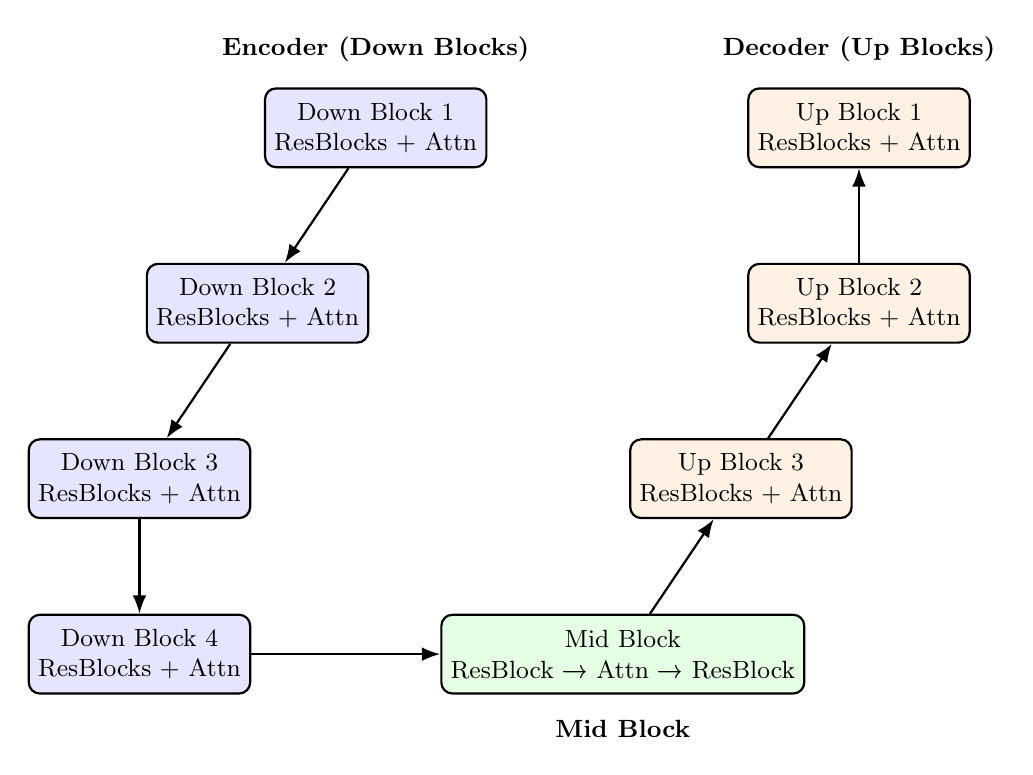
\begin{tikzpicture}[
    font=\small,
    block/.style={
        draw, thick, rounded corners,
        minimum width=2.6cm, minimum height=1cm,
        align=center
    },
    arrow/.style={-Latex, thick},
]

% ===============================
%         Down blocks (left)
% ===============================

\node[block, fill=blue!10] (down1) {Down Block 1\\ResBlocks + Attn};

\node[block, fill=blue!10, below=1.2cm of down1, xshift=-1.5cm] (down2)
    {Down Block 2\\ResBlocks + Attn};

\node[block, fill=blue!10, below=1.2cm of down2, xshift=-1.5cm] (down3)
    {Down Block 3\\ResBlocks + Attn};

\node[block, fill=blue!10, below=1.2cm of down3] (down4)
    {Down Block 4\\ResBlocks + Attn};


% ===============================
%          Mid block (bottom)
% ===============================

\node[block, fill=green!10, right=2.4cm of down4] (mid)
    {Mid Block\\ResBlock → Attn → ResBlock};


% ===============================
%         Up blocks (right)
% ===============================

\node[block, fill=orange!10, above=1.2cm of mid, xshift=1.5cm] (up3)
    {Up Block 3\\ResBlocks + Attn};

\node[block, fill=orange!10, above=1.2cm of up3, xshift=1.5cm] (up2)
    {Up Block 2\\ResBlocks + Attn};

\node[block, fill=orange!10, above=1.2cm of up2] (up1)
    {Up Block 1\\ResBlocks + Attn};


% ===============================
%              arrows
% ===============================

\draw[arrow] (down1) -- (down2);
\draw[arrow] (down2) -- (down3);
\draw[arrow] (down3) -- (down4);

\draw[arrow] (down4) -- (mid);

\draw[arrow] (mid) -- (up3);
\draw[arrow] (up3) -- (up2);
\draw[arrow] (up2) -- (up1);


% ===============================
%              labels
% ===============================

\node[above=0.2cm of down1] {\textbf{Encoder (Down Blocks)}};
\node[below=0.2cm of mid] {\textbf{Mid Block}};
\node[above=0.2cm of up1] {\textbf{Decoder (Up Blocks)}};

\end{tikzpicture}


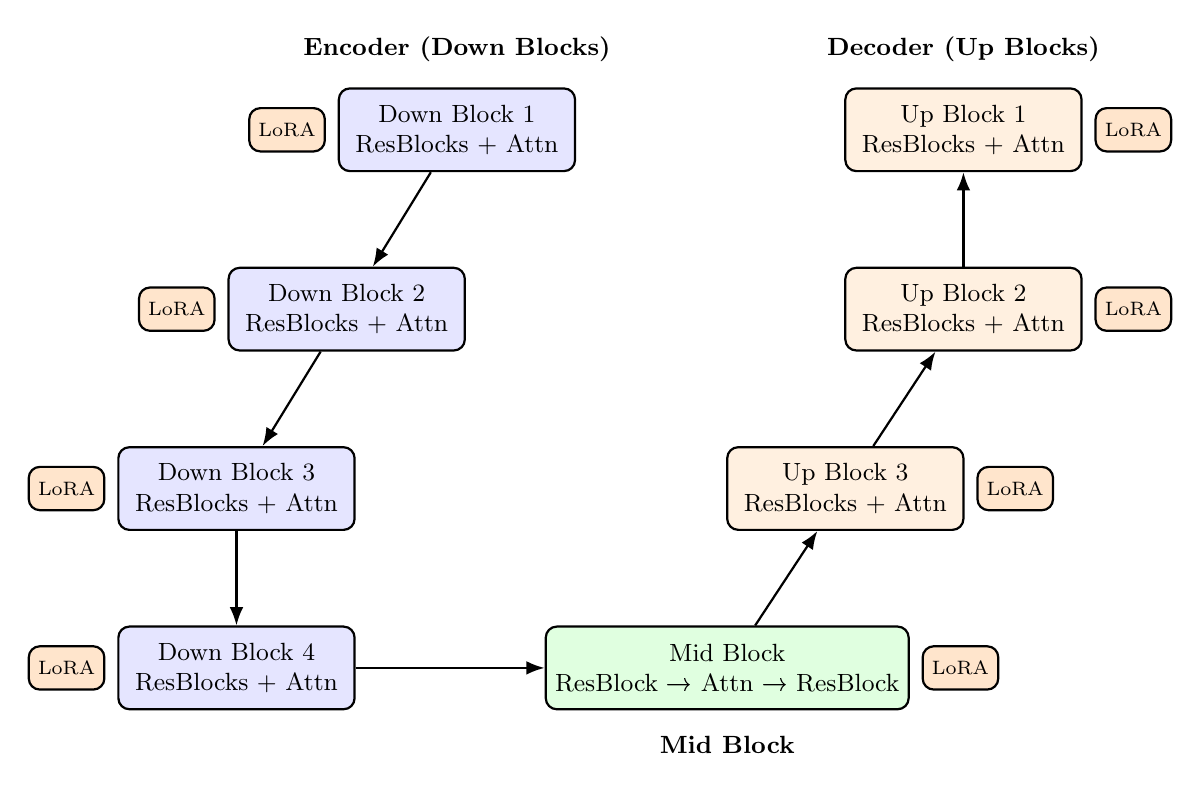
\begin{tikzpicture}[
    font=\small,
    block/.style={
        draw, thick, rounded corners,
        minimum width=3.0cm, minimum height=1.05cm,
        align=center
    },
    lorablock/.style={
        draw, thick, rounded corners,
        minimum width=0.9cm, minimum height=0.55cm,
        fill=orange!20,
        align=center,
        font=\scriptsize
    },
    arrow/.style={-Latex, thick},
]

% ============ Down Blocks ============

\node[block, fill=blue!10] (down1) {Down Block 1\\ResBlocks + Attn};
\node[lorablock, left=0.15cm of down1] (l1) {LoRA};

\node[block, fill=blue!10, below=1.2cm of down1, xshift=-1.4cm] (down2)
    {Down Block 2\\ResBlocks + Attn};
\node[lorablock, left=0.15cm of down2] (l2) {LoRA};

\node[block, fill=blue!10, below=1.2cm of down2, xshift=-1.4cm] (down3)
    {Down Block 3\\ResBlocks + Attn};
\node[lorablock, left=0.15cm of down3] (l3) {LoRA};

\node[block, fill=blue!10, below=1.2cm of down3] (down4)
    {Down Block 4\\ResBlocks + Attn};
\node[lorablock, left=0.15cm of down4] (l4) {LoRA};

% ============ Mid Block ============

\node[block, fill=green!12, right=2.4cm of down4] (mid)
    {Mid Block\\ResBlock → Attn → ResBlock};
\node[lorablock, right=0.15cm of mid] (lm) {LoRA};


% ============ Up Blocks ============

\node[block, fill=orange!12, above=1.2cm of mid, xshift=1.5cm] (up3)
    {Up Block 3\\ResBlocks + Attn};
\node[lorablock, right=0.15cm of up3] (lu3) {LoRA};

\node[block, fill=orange!12, above=1.2cm of up3, xshift=1.5cm] (up2)
    {Up Block 2\\ResBlocks + Attn};
\node[lorablock, right=0.15cm of up2] (lu2) {LoRA};

\node[block, fill=orange!12, above=1.2cm of up2] (up1)
    {Up Block 1\\ResBlocks + Attn};
\node[lorablock, right=0.15cm of up1] (lu1) {LoRA};


% ============ Arrows ============

\draw[arrow] (down1) -- (down2);
\draw[arrow] (down2) -- (down3);
\draw[arrow] (down3) -- (down4);

\draw[arrow] (down4) -- (mid);

\draw[arrow] (mid) -- (up3);
\draw[arrow] (up3) -- (up2);
\draw[arrow] (up2) -- (up1);

% Labels
\node[above=0.2cm of down1] {\textbf{Encoder (Down Blocks)}};
\node[below=0.2cm of mid] {\textbf{Mid Block}};
\node[above=0.2cm of up1] {\textbf{Decoder (Up Blocks)}};

\end{tikzpicture}




    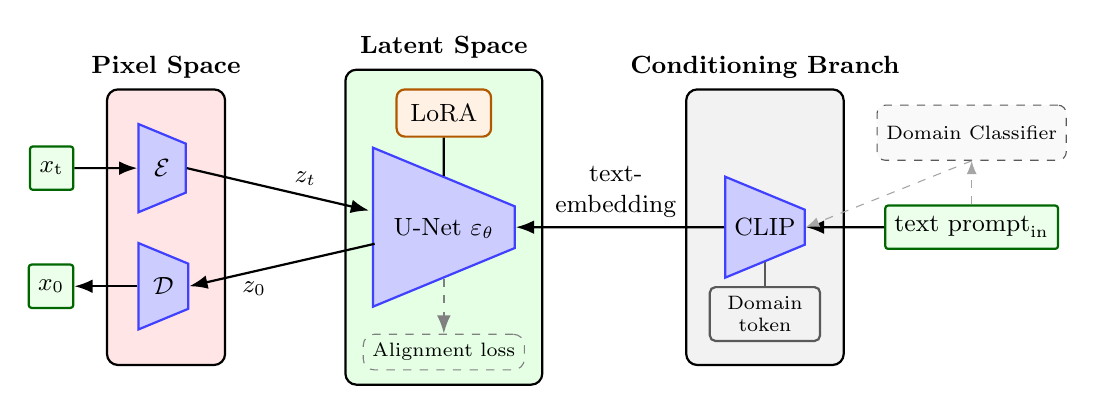
\begin{tikzpicture}[
    font=\small,
    >={Latex[length=3mm,width=2mm]}
]

% ===============================================================
% ==== Pixel Space ====
% ===============================================================
\node[module, fill=red!10, minimum width=1.5cm, minimum height=3.5cm,
      label=above:{\textbf{Pixel Space}}, align=center] (pixel) {};

% Encoder (右开口)
\node[mytrape={blue}{blue}, minimum width=1.1cm, minimum height=0.6cm, trapezium angle=67.5,
      right=0.4cm of pixel.west, shape border rotate=270, anchor=west, yshift=0.75cm] (enc) {$\mathcal{E}$};

% Decoder (左开口)
\node[mytrape={blue}{blue}, minimum width=1.1cm, minimum height=0.6cm, trapezium angle=67.5,
      shape border rotate=180, shape border rotate=270, right=0.4cm of pixel.west, anchor=west, yshift=-0.75cm] (dec) {$\mathcal{D}$};

\node[io, left=0.8cm of enc] (xenc) {$x_{\text{t}}$};
\node[io, left=0.8cm of dec] (xdec) {$x_{0}$};



% ===============================================================
% ==== Latent Space ====
% ===============================================================
\node[module, fill=green!10, minimum width=2.5cm, minimum height=4cm,
      right=1.5cm of pixel, label=above:{\textbf{Latent Space}}, align=center] (latent) {};

% === UNet 梯形 ===
% === UNet 梯形 (使用 mytrape 风格) ===
\node[mytrape={blue}{blue},
      minimum width=1.8cm,   % ← 宽度
      minimum height=1.8cm,% ← 高度
      shape border rotate=270,
      trapezium angle=67.5,
      trapezium stretches=false,
      anchor=center,
      at=(latent.center),
      text depth=-2ex, 
      text height=0.6em 
] (unet) {U-Net $\varepsilon_\theta$};

% 箭头
% 输入 -> Encoder
\draw[-Latex, thick] (xenc) -- (enc);

% ===== 上方 Encoder → UNet =====
\draw[-Latex, thick]
    (enc.east) -- ([xshift=-1pt, yshift=6pt]unet.west)
    node[pos=0.65, above, font=\small]{$z_t$};

% ===== UNet → 下方 Decoder =====
\draw[-Latex, thick]
    ([xshift=1pt, yshift=-6pt]unet.west) -- (dec.east)
    node[pos=0.65, below, font=\small]{$z_0$};

% Decoder -> 输出
\draw[-Latex, thick] (dec.west) -- (xdec);


% === LoRA 方块 ===
\node[
    draw=orange!70!black, fill=orange!10,
    rounded corners=3pt, thick,
    minimum width=1.2cm, minimum height=0.6cm,
    font=\small
] (lora) at ([yshift=1.45cm]unet.center) {LoRA};

% === 连接线
\draw[thick, black]
    (unet.north) -- (lora.south);
    
% === Alignment loss ===
\node[
    draw=gray, dashed, rounded corners,
    below=0.7cm of unet, font=\scriptsize
] (align) {Alignment loss};
\draw[dashed, gray, thick, -Latex] (unet.south) -- (align.north);


% ===============================================================
% ==== Conditioning Branch ====
% ===============================================================
\node[module,
      fill=gray!10,
      minimum width=2cm,
      minimum height=3.5cm,
      right=1.8cm of latent,
      label=above:{\textbf{Conditioning Branch}},
      align=center
] (cond) {
};

\node[io, right=0.5cm of cond] (textprompt) {$\text{text prompt}_{\text{in}}$};

% === CLIPencoder ===
\node[mytrape={blue}{blue},
      minimum width=1cm,
      minimum height=1cm,
      shape border rotate=270,
      trapezium angle=67.5,
      trapezium stretches=false,
      anchor=center,
      at=(cond.center),
      text height=0.6em,
      align=center  % ← 允许换行
] (clipencoder) {CLIP};

\node[
    draw=gray!70!black,
    fill=gray!10,
    rounded corners=2pt,
    thick,
    minimum width=1.4cm,
    minimum height=0.3cm,
    below=0.3cm of clipencoder,
    font=\scriptsize,
    align=center
] (domaintoken) {Domain\\token};

% domain classifier
% === Domain Classifier ===
\node[
    draw=gray!70!black,
    dashed,
    fill=gray!05,
    rounded corners=3pt,
    minimum width=2.1cm,
    minimum height=0.7cm,
    font=\scriptsize
] (domaincls) at ($(textprompt) + (0,1.2)$) {Domain Classifier};



% 加一条线连接到 CLIP encoder
\draw[thick, gray!70!black] (domaintoken.north) -- (clipencoder.south);

\draw[-Latex, thick] (clipencoder.west) -- node[above, midway, pos=0.52, align=center, text width=2cm]{text-embedding} (unet.east);
\draw[-Latex, thick] (textprompt.west) -- (clipencoder.east);
% % text prompt → Domain Classifier
% \draw[-Latex, thick] (textprompt.west) -- (domaincls.south);

% % Domain Classifier → CLIP
% \draw[-Latex, thick] (domaincls.south) -- (clipencoder.east);
% text prompt → Domain Classifier (dashed arrow)
\draw[dashed, -Latex, gray!70] (textprompt.north) -- (domaincls.south);

% Domain Classifier → CLIP (dashed arrow)
\draw[dashed, -Latex, gray!70] (domaincls.south) -- (clipencoder.east);


\end{tikzpicture}

\end{document}
